% Shared SPI bus (firmware/isingmachine/src/board.h, drivers/bus.cpp, hcs165.cpp, mcp4351.cpp).
% CS1 (GPIO 21) enables the SN74HCS138 3-8 decoder (U13); ADDR0-2 (GPIO 15, 33, 27) pick its output.
%   Address 0-6: DP_CS0-6 low selects one MCP4351 digipot (U16-U22) to program its four coupler wipers (SPI mode 0).
%   Address 7:   CLK_INH low ungates SCLK into the SN74HCS165 (U15) and switches the MISO mux to its QH.
%                SH/LD (GPIO 19) rising latches WIN_A..WIN_H at once; 8 clocks shift them out (SPI mode 2).
% Build: lualatex spi-bus.tex && pdftoppm -png -r 300 -singlefile spi-bus.pdf spi-bus
\documentclass[border=8pt]{standalone}
\usepackage{tikz}
\usetikzlibrary{arrows.meta}
\usepackage{fontspec}
\setmainfont{TeX Gyre Heros}
\usepackage{sansmath}
\sansmath


\begin{document}
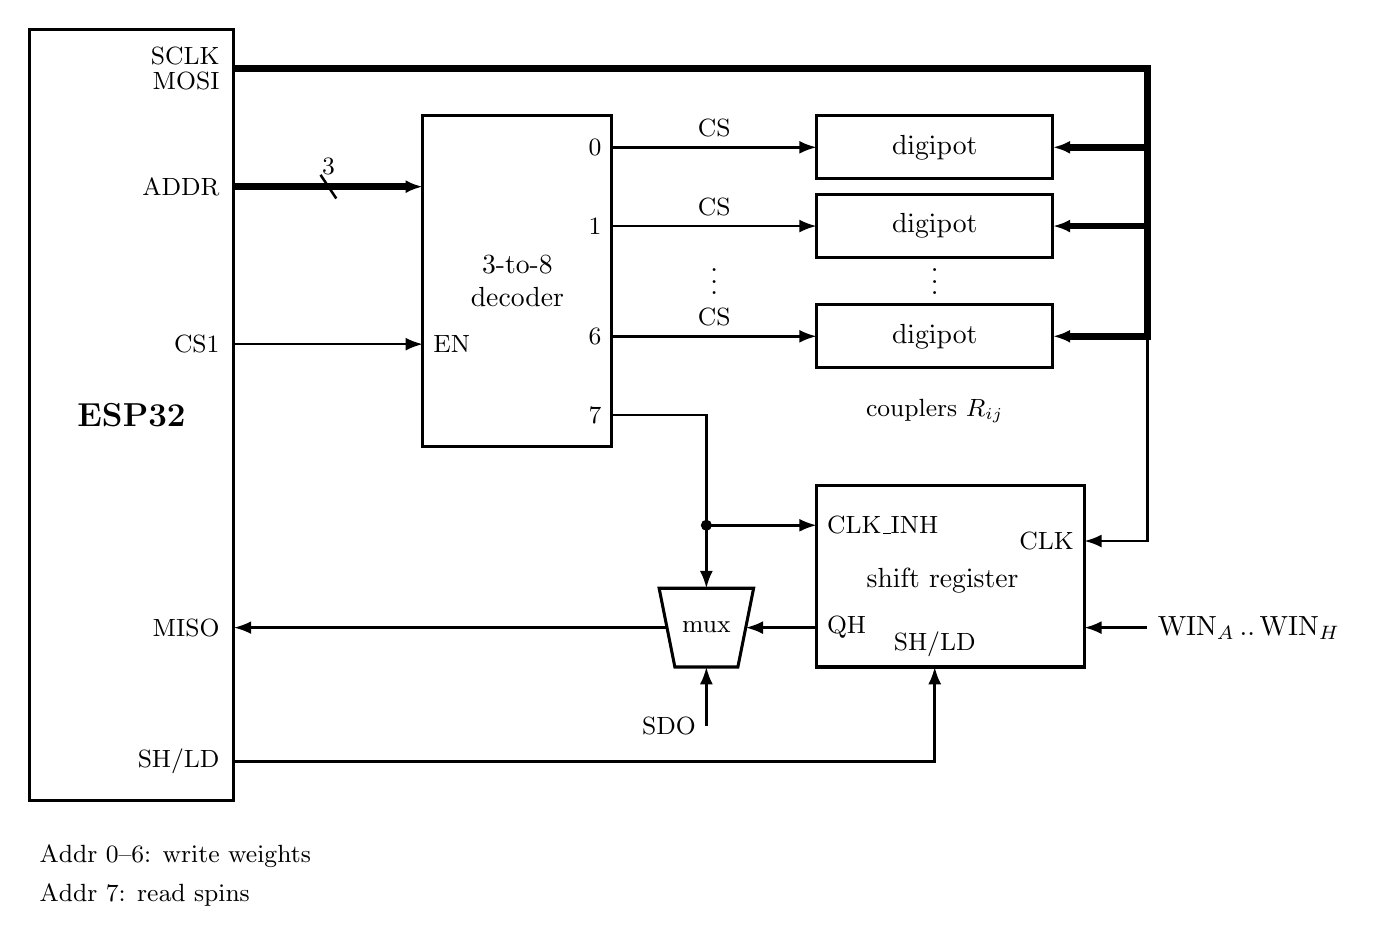
\begin{tikzpicture}[
    font=\normalsize, line width=0.9pt, >={Latex[length=2.2mm]},
    chip/.style={draw, line width=1.1pt, fill=white, align=center},
    pin/.style={font=\small},
    bus/.style={line width=2.4pt},
  ]
  % ESP32
  \draw[chip] (0,0.5) rectangle (2.6,-9.3);
  \node[font=\large\bfseries] at (1.3,-4.4) {ESP32};
  \foreach \y/\t in {0/SCLK\\[-2pt]MOSI, -1.5/ADDR, -3.5/CS1, -7.1/MISO, -8.8/{SH/LD}}
    \node[pin, anchor=east, align=right] at (2.55,\y) {\t};

  % Shift register (drawn first so pin labels sit on top)
  \draw[chip] (10,-5.3) rectangle (13.4,-7.6);
  \node[align=center] at (11.6,-6.5) {shift register};

  % SPI bus: SCLK + MOSI to the digipots, SCLK to the shift register
  \draw[bus, ->] (2.6,0) -- (14.2,0) -- (14.2,-1.0) -- (13,-1.0);
  \draw[bus, ->] (14.2,-1.0) -- (14.2,-2.0) -- (13,-2.0);
  \draw[bus, ->] (14.2,-2.0) -- (14.2,-3.4) -- (13,-3.4);
  \draw[->] (14.2,-3.4) -- (14.2,-6.0) -- (13.4,-6.0) node[pin, left] {CLK};

  % 3-8 decoder
  \draw[chip] (5,-0.6) rectangle (7.4,-4.8);
  \node[align=center] at (6.2,-2.7) {3-to-8\\decoder};
  \draw[bus, ->] (2.6,-1.5) -- node[above, pin] {3} (5,-1.5);
  \draw (3.7,-1.35) -- (3.9,-1.65);
  \draw[->] (2.6,-3.5) -- (5,-3.5) node[pin, right] {EN};

  % Addresses 0-6: one digipot chip select each
  \foreach \y/\a in {-1.0/0, -2.0/1, -3.4/6} {
    \draw[->] (7.4,\y) node[pin, left] {\a} -- node[pin, above] {CS} (10,\y);
    \draw[chip] (10,\y+0.4) rectangle (13,\y-0.4);
    \node at (11.5,\y) {digipot};
  }
  \node at (11.5,-2.6) {$\vdots$};
  \node at (8.7,-2.6) {$\vdots$};
  \node[font=\small, align=center] at (11.5,-4.35) {couplers $R_{ij}$};

  % Address 7: CLK_INH to the shift register and the MISO mux select
  \draw[->] (7.4,-4.4) node[pin, left] {7} -- (8.6,-4.4) -- (8.6,-5.8) -- (10,-5.8) node[pin, right] {CLK\_INH};
  \fill (8.6,-5.8) circle (2pt);
  \draw[->] (8.6,-5.8) -- (8.6,-6.6);

  % Shift register
  \draw[<-] (13.4,-7.1) -- ++(0.8,0) node[right] {WIN$_A$\,..\,WIN$_H$};
  \draw[->] (2.6,-8.8) -- (11.5,-8.8) -- (11.5,-7.6) node[pin, above] {SH/LD};

  % MISO mux: digipot SDO, or QH when CLK_INH is low
  \draw[chip] (8.0,-6.6) -- (9.2,-6.6) -- (9.0,-7.6) -- (8.2,-7.6) -- cycle;
  \node[font=\small] at (8.6,-7.1) {mux};
  \draw[->] (10,-7.1) node[pin, right] {QH} -- (9.1,-7.1);
  \draw[->] (8.6,-8.35) node[pin, left] {SDO} -- (8.6,-7.6);
  \draw[->] (8.1,-7.1) -- (2.6,-7.1);

  % What each address does
  \node[anchor=west, font=\small] at (0,-10.0) {Addr 0--6: write weights};
  \node[anchor=west, font=\small] at (0,-10.5) {Addr 7: read spins};
\end{tikzpicture}
\end{document}
